\documentclass[11pt,a4paper,oneside]{report}
\usepackage[ngerman]{babel}
% \usepackage{url} or \usepackage{hyperref}
\usepackage[utf8]{inputenc} % Displays German 'Umlaute' correctly. Also some workaround, see Bibliography Management#BibTeX in wikibooks
\usepackage{graphicx}
%\usepackage{titlesec}

\setcounter{secnumdepth}{3}
\setcounter{tocdepth}{5}

\addto{\captionsngerman}{\renewcommand*{\abstractname}{Abstract}}
%\renewcommand{\abstractname}{Abstract}

\newcommand{\thema}{Sicherheitsbetrachtungen von Applikations-Containersystemen in Cloud-Infrastukturen am Beispiel Docker}
\newcommand*{\signatureAndDate}{
    \par\noindent\makebox[2.5in]{\hrulefill} \hfill\makebox[2.0in]{\hrulefill}%
    \par\noindent\makebox[2.5in][l]{Unterschrift}      \hfill\makebox[2.0in][l]{Datum}%
}

\begin{document}

\begin{titlepage}
	\centering
	% \includegraphics[width=0.15\textwidth]{example-image-1x1}\par\vspace{1cm}
	{\scshape\LARGE
		Hochschule der Medien
	\par}
	\vspace{1cm}
	{\scshape\Large
		Bachelorarbeit
	\par}
	\vspace{1.5cm}
	{\huge\bfseries
		\thema
	\par}
	\vspace{2cm}
	{\Large\itshape
		Moritz Hoffmann
	\par}
	\vspace{0.5cm}
	{\Large
		Studiengang: Mobile Medien\\
		Matrikelnummer: 26135\\
		E-Mail: \texttt{mh203@hdm-stuttgart.de}
	\par}
	\vspace{1.5cm}
	{\Large Dezember 2015\par}
	% Bottom of the page
	\vfill
	{\Large
		\emph{Erstbetreuer:}\hfill\emph{Zweitbetreuer:}\\
		Prof. Dr. Joachim Charzinski\hfill Patrick Fröger\\
		Hochschule der Medien\hfill ITI/GN, Daimler AG
	\par}

\end{titlepage}


\title{\thema}
\author{Moritz Hoffmann\\
  Studiengang Mobile Medien,\\
  Hochschule der Medien\\
  \texttt{mh203@hdm-stuttgart.de}}
\date{Dezember 2015}
% \date{\today}
\maketitle

\chapter*{Eidesstattliche Erklärung}
\emph{„Hiermit versichere ich, Moritz Hoffmann, ehrenwörtlich, dass ich die vorliegende Bachelorarbeit mit dem Titel: „\thema“ selbstständig und ohne fremde Hilfe verfasst und keine anderen als die angegebenen Hilfsmittel benutzt habe. Die Stellen der Arbeit, die dem Wortlaut oder dem Sinn nach anderen Werken entnommen wurden, sind in jedem Fall unter Angabe der Quelle kenntlich gemacht. Die Arbeit ist noch nicht veröffentlicht oder in anderer Form als Prüfungsleistung vorgelegt worden. Ich habe die Bedeutung der ehrenwörtlichen Versicherung und die prüfungsrechtlichen Folgen (§26 Abs. 2 Bachelor-SPO (6 Semester), § 24 Abs. 2 Bachelor-SPO (7 Semester), § 23 Abs. 2 Master-SPO (3 Semester) bzw. § 19 Abs. 2 Master-SPO (4 Semester und berufsbegleitend) der HdM) einer unrichtigen oder unvollständigen ehrenwörtlichen Versicherung zur Kenntnis genommen.“
}
\vspace{1.5cm}
\signatureAndDate
\newpage


% Abstract
\begin{abstract}
\noindent\emph{English version:}\newline\newline
\noindent
....\\
..\\

\vspace{1cm}
\noindent\emph{Deutsche Version:}\newline\newline
\noindent
....\\
...\\
.\\
..\\

\end{abstract}

% Table of Contents
\tableofcontents

% Abbildungsverzeichnis
\listoffigures

% Tabellenverzeichnis
\listoftables

% \linespread{1.3}            % 1.5x line spacing
% \linespread{1.6}            % Double line spacing
% \hfill test                 % insert horizontal stretched space
% \vfill test                 % insert vertical stretched space
% ,,German quotation marks``  % deutsche Anfuehrungszeichen

% this is a comment
Hallo %\cite{myquote1}
One more line %\cite[S.2]{myquote1,myquote2}
jooooo \cite{Senn2009}

\begin{figure}[h] % with [p], images is displayed on own page
    \centering
    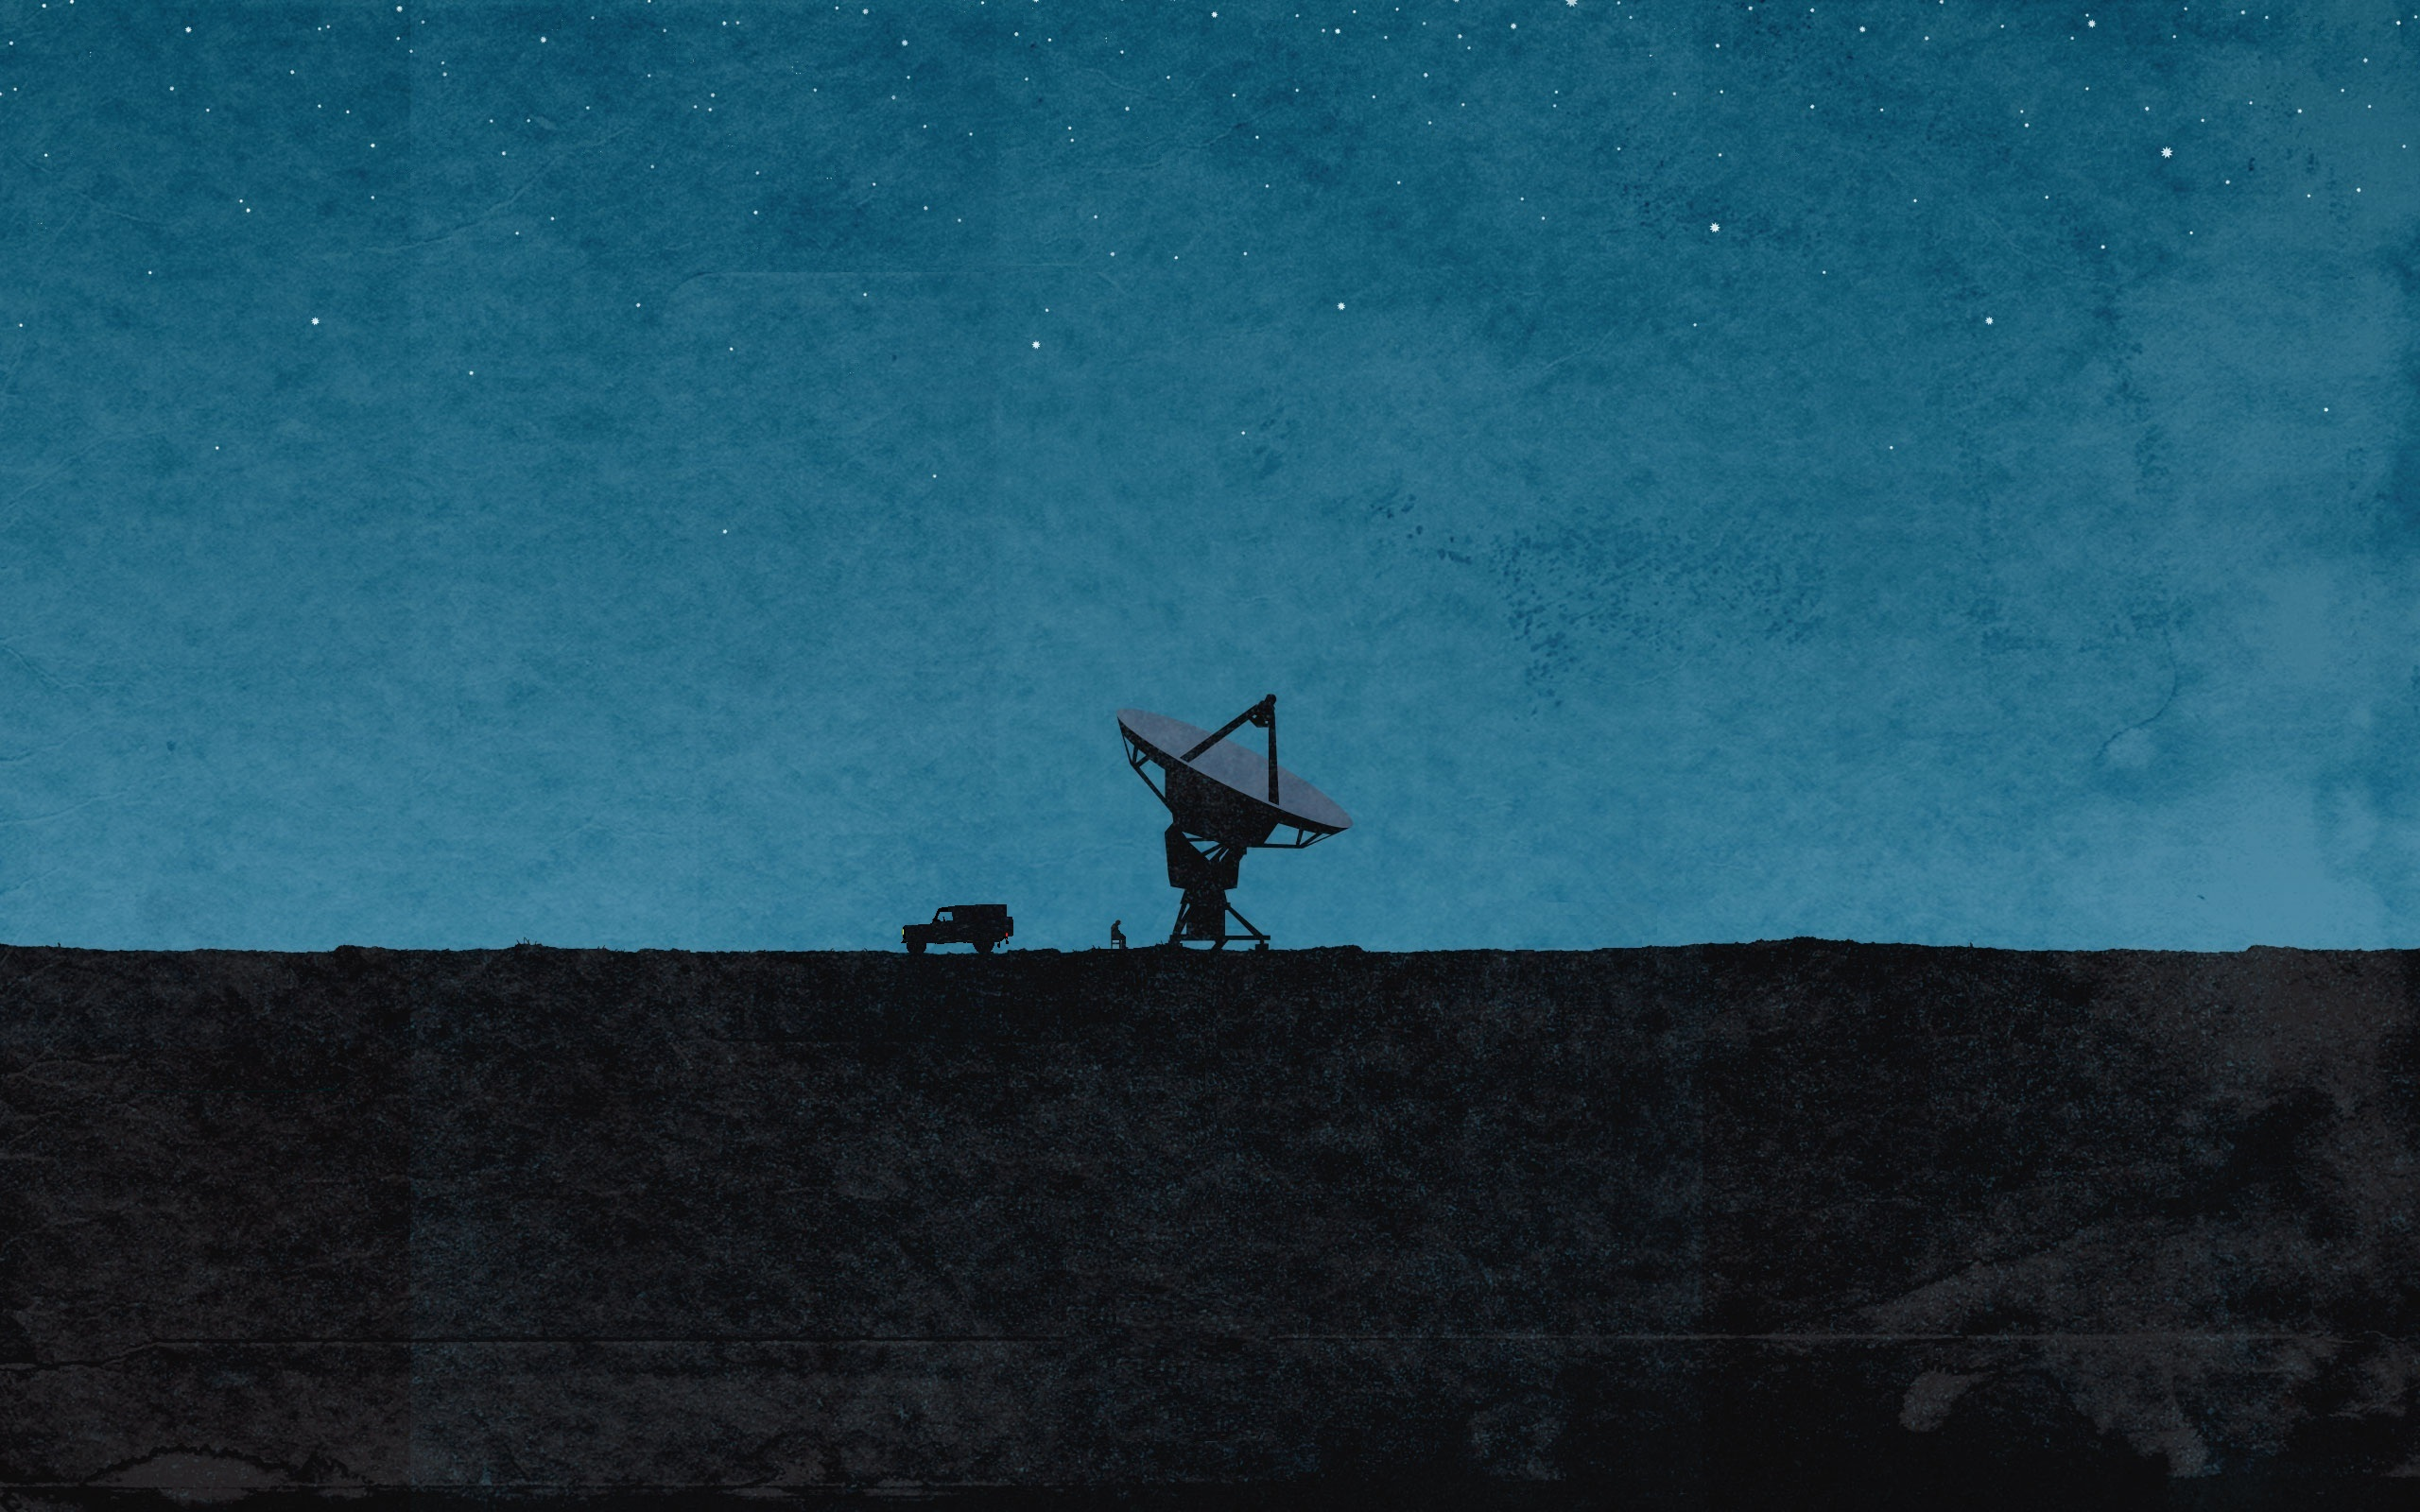
\includegraphics[width=1.0\textwidth]{./images/image.jpg}
    \caption{Awesome Image}
    \label{fig:awesome_image}
\end{figure}

lkasjdflkj asldkjf lasjkdflkadsjf ladksjflkjslkdjf    dslfjklaks df a sdfjaldsfj  ladksjf lkjlakjsd f asdf aljsdflkjasldfjalsdfj l adskjflj d f dslkfjalksdjf sd fljsdfkjsld f

\emph{dieser text ist kursiv}

asdfasdfasdfasdlkvalrkgjval  asdkfj  sldkfjlsdjfa adaher is kes ji lkaskdj ladskj a ldksfjll aldkfj lkj afsdlfkjl alsdkf jaldskfj la sdflaldsflas df sadfl sf

\texttt{das hier ist monotype}

% TODO: reformat chapter style with package titlesec
%\titleformat{\section}
%{\filcenter\normalfont\Large\bfseries}
%{\chaptertitlename~\thechapter} {0.5em} {}


% GLIEDERUNG
\chapter{Überblick}
	\section{Arten von Virtualisierungen}
	  \subsection{Einordnung Docker}
  \section{Einführung in Docker}
  % @Charzinski: Ist es OK das erste kapitel zu untergliedern? Oder besser separate chapters um Docker zu erklären?
\chapter{Ziel der Arbeit/Forschungsfrage}
  % Kommt man von Container auf Host-OS? Von Container auf anderen Container? ~etc.
  % 5-6 Sicherheitsziele erwähnen. Mit Forschungsfrage in Bezug bringen --> später bei Isolierung und Ressourcenverwaltung wieder aufgreifen
\chapter{Security aus Linux Kernel-Features}
  % namespaces/etc (was es ist) in Einleitung mit rein? 1.) Erklaeren, 2.) Security/Docker untersuchen dazu im Security Hauptteil
  % 2 Unterkapitel, inhatliche Überschneidung evtl., Grund nennen warum so gegliedert, ...
	\section{Isolierung}
    % Isolierung erklären, erfüllt X Schutzziele, Bezug auf Forschungsfrage
		\subsection{\texttt{namespaces}}
			\subsubsection{\texttt{user namespaces}}
      % Future implementation, da sehr neu. Trotzdem Konzept erklären und wie Docker-Security davon profitiert.
		\subsection{\texttt{capabilities}}
			\subsubsection{Beispiele, \texttt{/proc}-Verzeichnis, (Un-)Mounten des Host-Filesystems}
      % Gehört das unter 'capabilities'? Oder eigener Punkt bzw. woanders dazu?
		\subsection{Mandatory Access Control (MAC)}
			\subsubsection{Beispiel SELinux}
      % Macht Sinn das erst am Ende zu machen, wenn noch Zeit ist. Weil SELinux im Detail mehr Exkurs wird.
	\section{Ressourcenverwaltung}
    % Sicherheitsziel: Availability, Bezug auf Forschungsfrage
    % Ressourcenverteilung und -management
    % Storage, CPU, HDD, RAM, IO, Network
		\subsection{\texttt{cgroups}}
	\section{Docker im Vergleich zu anderen Containerlösungen}
  % Mandatory?
\chapter{Security im Docker-Ökosystem}
  % ### Hier mit Patrick weitermachen ###
  % Je nach Vorankommen, können hier ganze Sektions weggelassen werden imo.
  % Tendenziell mehr die Themen zuerst, die direkt mit Security zu tun haben.
  \section{Docker Images und Repositories}
		\subsection{neues Signierungs-Feature}
	\section{Docker Daemon}
		\subsection{REST-API}
		\subsection{Support von Zertifikaten}
	\section{Docker Cache}
	\section{\texttt{privileged} Container}
	\section{Networking}
		\subsection{\texttt{bridge} Netzwerk}
		\subsection{\texttt{overlay} Netzwerk}
		\subsection{DNS}
		\subsection{Portmapping}
	\section{Daten-Container}
	\section{Docker mit VMs}
	\section{Tools rund um Docker}
		\subsection{Docker Swarm}
		\subsection{Docker Compose}
		\subsection{Nautilus Project}
		\subsection{Vagrant}
		\subsection{Kubernetes}
\chapter{Docker in Unternehmen/Clound-Infrastrukturen}
% Wichtiges Kapitel für Daimler, mein Chef, Management
% Kapitel, das erst angegangen wird, wenn min. Kapitel 1 steht (Januar 2016 oder später).

% ???: Transscript aus Besprechung mit Herr Fahner und Patrick:
% Welche Security-Features uebernimmt die Cloud, welche muss Docker gewaehrleisten. Was
% bieten MS Azure/Amazon's AWS/etc fuer Mechanismen an?
% Welche Möglichkeiten zur sicheren Docker-Integration bieten diese?
% Wortlaut Patrick: Wie funktionierts bei Azure, wie funktionierts wenn man es
% selbst implementiert.
\chapter{Fazit/Ausblick}
% Wenig Angriffsvektoren auf Docker/Container bekannt. "Sichergehen" kann man nur mit Konzepten wie "Docker in VMs" und "VMs in Docker".
% neuste Docker-Releases und deren Fokus (Enterprise,Production-Readiness,Security)
% seit Juli 2015 ist standardisiertes Containerformat der big player in Arbeit
% Ausblick im Kontext von Container VS. konventioneller Virtualisierung

%\subsection{Subsektion blabla}
%\subsubsection{Subsubsektion blablabla}
%\paragraph{Paragraph soundso}
%\subparagraph{SubParagraph soundso}



% Anhang
\appendix

% Bibliography
\bibliographystyle{plain}
\bibliography{test} % specify name of bibfile

\end{document}
